\chapter{Introduction}

Let me introduce to the topic of my PhD 

Design, manufacturing and developing software for an omnidirectional agricultural robot.

The solution comes in the form of a 4-wheeled robot 

The proposed solution comprises the following modules:

\begin{itemize}
    \item chassis
    \item wheel base
    \item electrics
    \item sensing, computation and communication
    \item software
\end{itemize}

The software could in turn be broken down into the following:

\begin{itemize}
    \item data transport
    \item localization
    \item target CV problem
    \item logging and data representation
    \item path planning
    \item user interface
\end{itemize}

Let us describe each of the elements of the system in detail.

chassis

The main structural elements of the robot's frame are manufactured from the aluminum profile (tube with rectangular cross-section).
They were designed to withstand the loads that exceed the normal ones with a huge margin.
The rigidity is assured by a rectangular section of a composite material (alucobond) that separates the inner volume of the robot into two.
The tubes were connected by flat milled aluminum elements.
The assembly was performed using bolts and nuts, as well as rivets and bits of welding.
The total weight of the chassis if N \si{kg}.

wheel base

The wheels were designed to work in pairs: each omnidirectional wheel is mechanically coupled with a rail wheel

electrics



sensing, computation and communication



software



data transport



localization



target CV problem



logging and data representation



path planning



user interface



\todo[inline]{TODO: complete chapter}

\section{Thesis Structure}
The diagram in \ref{fig:thesis-structure} illustrates the flow of information through the structure of the thesis.



\begin{figure}[htb!]
\centering 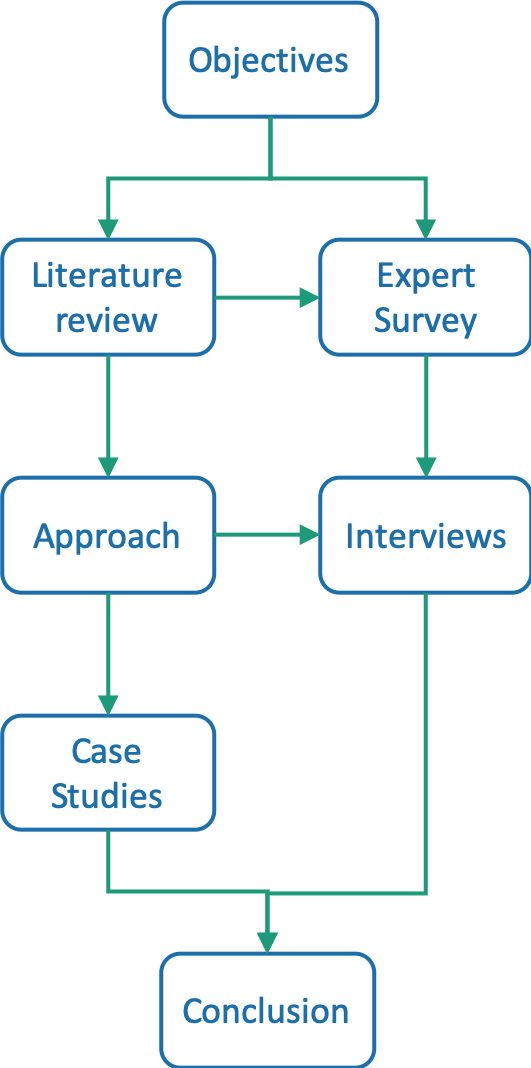
\includegraphics[width=0.5\textwidth]{graphics/thesis-structure}
\caption{Thesis structure}
\label{fig:thesis-structure}
\end{figure}

\begin{description}
    \item[\ref{cap:background} - Background]
Here's the literature review.

    \item[\ref{cap:thesis_objectives} - Thesis Objectives]
We define the objectives of our work.

...

    \item[\ref{cap:conclusion} - Conclusion]
In the last chapter, we discuss our results obtained ...

\end{description}

